% 这是中国科学院大学计算机科学与技术专业《计算机组成原理(研讨课)》使用的实验报告 Latex 模板
% 本模板与 2024 年 2 月 Jun-xiong Ji 完成, 更改自由 Shing-Ho Lin 和 Jun-Xiong Ji 于 2022 年 9 月共同完成的基础物理实验模板
% 如有任何问题, 请联系: jijunxoing21@mails.ucas.ac.cn
% This is the LaTeX template for report of Experiment of Computer Organization and Design courses, based on its provided Word template. 
% This template is completed on Febrary 2024, based on the joint collabration of Shing-Ho Lin and Junxiong Ji in September 2022. 
% Adding numerous pictures and equations leads to unsatisfying experience in Word. Therefore LaTeX is better. 
% Feel free to contact me via: jijunxoing21@mails.ucas.ac.cn

\documentclass[11pt]{article}

\usepackage[a4paper]{geometry}
\geometry{left=2.0cm,right=2.0cm,top=2.5cm,bottom=2.5cm}

\usepackage{ctex} % 支持中文的LaTeX宏包
\usepackage{amsmath,amsfonts,graphicx,subfigure,amssymb,bm,amsthm,mathrsfs,mathtools,breqn} % 数学公式和符号的宏包集合
\usepackage{algorithm,algorithmicx} % 算法和伪代码
\usepackage[noend]{algpseudocode} % 算法和伪代码
\usepackage{fancyhdr} % 自定义页眉页脚
\usepackage[framemethod=TikZ]{mdframed} % 创建带边框的框架
\usepackage{fontspec} % 字体设置
\usepackage{adjustbox} % 调整盒子大小
\usepackage{fontsize} % 设置字体大小
\usepackage{tikz,xcolor} % 绘制图形和使用颜色
\usepackage{multicol} % 多栏排版
\usepackage{multirow} % 表格中合并单元格
\usepackage{pdfpages} % 插入PDF文件
\usepackage{listings} % 在文档中插入源代码
\usepackage{wrapfig} % 文字绕排图片
\usepackage{bigstrut,multirow,rotating} % 支持在表格中使用特殊命令
\usepackage{booktabs} % 创建美观的表格
\usepackage{circuitikz} % 绘制电路图
\usepackage{zhnumber} % 中文序号(用于标题)
\usepackage{tabularx} % 表格折行

\definecolor{dkgreen}{rgb}{0,0.6,0}
\definecolor{gray}{rgb}{0.5,0.5,0.5}
\definecolor{mauve}{rgb}{0.58,0,0.82}
\lstset{
  frame=tb,
  aboveskip=3mm,
  belowskip=3mm,
  showstringspaces=false,
  columns=flexible,
  framerule=1pt,
  rulecolor=\color{gray!35},
  backgroundcolor=\color{gray!5},
  basicstyle={\small\ttfamily},
  numbers=none,
  numberstyle=\tiny\color{gray},
  keywordstyle=\color{blue},
  commentstyle=\color{dkgreen},
  stringstyle=\color{mauve},
  breaklines=true,
  breakatwhitespace=true,
  tabsize=3,
}

% 轻松引用, 可以用\cref{}指令直接引用, 自动加前缀. 
% 例: 图片label为fig:1
% \cref{fig:1} => Figure.1
% \ref{fig:1}  => 1
\usepackage[capitalize]{cleveref}
% \crefname{section}{Sec.}{Secs.}
\Crefname{section}{Section}{Sections}
\Crefname{table}{Table}{Tables}
\crefname{table}{Table.}{Tabs.}

% \setmainfont{Palatino Linotype.ttf}
% \setCJKmainfont{SimHei.ttf}
% \setCJKsansfont{Songti.ttf}
% \setCJKmonofont{SimSun.ttf}
\punctstyle{kaiming}
% 偏好的几个字体, 可以根据需要自行加入字体ttf文件并调用

\renewcommand{\emph}[1]{\begin{kaishu}#1\end{kaishu}}

% 对 section 等环境的序号使用中文
\renewcommand \thesection{\zhnum{section}、}
\renewcommand \thesubsection{\arabic{section}}


%%%%%%%%%%%%%%%%%%%%%%%%%%%
%改这里可以修改实验报告表头的信息
\newcommand{\name}{艾华春, 李霄宇, 王敬华}
\newcommand{\studentNum}{2022K8009916011,2022K8009929029,2022K8009925009}
\newcommand{\major}{计算机科学与技术}
\newcommand{\labNum}{4}
\newcommand{\labName}{异常和中断的支持}
%%%%%%%%%%%%%%%%%%%%%%%%%%%

\begin{document}

\begin{center}
  \LARGE \bf 中国科学院大学 \\《计算机体系结构基础(研讨课)》实验报告
\end{center}

\begin{center}
  \emph{姓名} \underline{\makebox[10em][c]{\name}} \\
  % 如果名字比较长, 可以修改box的长度"8em"为其他值
  \emph{学号} \underline{\makebox[30em][c]{\studentNum}}\\
  % \emph{专业} \underline{\makebox[15em][c]{\major}}\\
  \emph{实验项目编号} \underline{\makebox[3em][c]{\labNum}}
  \emph{实验名称} \underline{\makebox[30em][c]{\labName}}\\
\end{center}

% \begin{center}
%   \begin{tabularx}{\textwidth}{|lX|}
%     \hline
%     注1: & 撰写此 Word 格式实验报告后以 PDF 格式保存 SERVE CloudIDE 的 \texttt{/home/serve-ide/ cod-lab/reports} 目录下(注意:reports 全部小写)。文件命名规则:\texttt{prjN.pdf},其中 \texttt{prj} 和后缀名 \texttt{pdf} 为小写,\texttt{N} 为1至4的阿拉伯数字。例如:\texttt{prj1.pdf}。PDF 文件大小应控制在 5MB 以内。此外,实验项目5包含多个选做内容,每个选做实验应提交各自的实验报告文件,文件命名规则:\texttt{prj5-projectname.pdf},其中``-''为英文标点符号的短横线。文件命名举例:\texttt{prj5-dma.pdf}。具体要求详见实验项目5讲义。 \\

%     注2: & 使用\texttt{git add}及\texttt{git commit}命令将实验报告\texttt{PDF}文件添加到本地仓库master分支,并通过\texttt{git push}推送到实验课SERVE GitLab远程仓库master分支(具体命令详见实验报告)。 \\

%     注3: & 实验报告模板下列条目仅供参考,可包含但不限定如下内容。实验报告中无需重复描述讲义中的实验流程。\\
%     \hline
%   \end{tabularx}
% \end{center}

  

\section{逻辑电路结构与仿真波形的截图及说明}
\noindent
$\bullet$
\textbf{添加系统调用异常支持}。
\begin{enumerate}
  \item 添加控制寄存器CRMD, PRMD, ESTAT, ERA, EENTRY, SAVE0-3
  
  新建一个csrfile的模块,里面包括所有控制寄存器的实现,并在\verb|mycpu_top|中进行例化,与各个流水级处于并列地位。

  模块接口包括两类,用于指令访存的接口和与处理器硬件电路逻辑直接交互的接口。

  \begin{table}[!ht]
    \centering
    \begin{tabular}{|l|l|l|l|l|}
    \hline
        接口名称 & 接口类型 & 含义 & 位宽 & 输入或输出 \\ \hline
        csr\_re & 指令访问 & 读使能 & 1 & input \\ \hline
        csr\_num & 指令访问 & 寄存器号 & 14 & input \\ \hline
        csr\_rvalue & 指令访问 & 寄存器返回值 & 32 & output \\ \hline
        csr\_we & 指令访问 & 写使能 & 1 & input \\ \hline
        csr\_wmask & 指令访问 & 写掩码 & 32 & input \\ \hline
        csr\_wvalue & 指令访问 & 写数据 & 32 & input \\ \hline
        wb\_ex & 硬件电路交互 & 异常处理触发信号 & 1 & input \\ \hline
        wb\_ecode & 硬件电路交互 & 异常类型 & 6 & input \\ \hline
        wb\_esubcode & 硬件电路交互 & 异常类型 & 9 & input \\ \hline
        wb\_pc & 硬件电路交互 & 触发异常的pc值 & 32 & input \\ \hline
        wb\_vaddr & 硬件电路交互 & 触发异常的虚地址 & 32 & input \\ \hline
        ertn\_flush & 硬件电路交互 & ertn指令 & 1 & input \\ \hline
        .... & ~ & ~ & ~ & ~ \\ \hline
    \end{tabular}
\end{table}
在写回级流水级模块wb\_reg中,创建上述所有的接口。
在cpu\_top模块中,将两个模块wb\_reg和csrfile中对应的接口相连接。

最后,在csrfile模块中创建了所有输入输出接口后,按照讲义上的内容,以每个CSR的各个域作为基本单位,
依次实现各个控制寄存器初始化,被指令访问和修改,被硬件电路逻辑访问和修改。

\item 增加控制寄存器ECFG, BADV, TID, TCFG, TVAL, TICLR

补全ECFG和BADV寄存器。
\begin{lstlisting}[language=verilog]
/*---------------------------ECFG---------------------------------------------------*/
always @(posedge clk)begin
    if(~resetn)
        csr_ecfg_lie <= 13'b0;
    else if (csr_we && csr_num == `CSR_ECFG)            // csr_ecfg_lie[10] == 0 
        csr_ecfg_lie <=     csr_wmask[`CSR_ECFG_LIE] & 13'h1bff & csr_wvalue[`CSR_ECFG_LIE]
                            | ~csr_wmask[`CSR_ECFG_LIE] & 13'h1bff & csr_ecfg_lie;
end
/*---------------------------ERA---------------------------------------------------*/
always @(posedge clk)begin
    if(wb_ex)
        csr_era_pc <=       wb_pc;
    else if(csr_we && csr_num == `CSR_ERA)
        csr_era_pc <=       csr_wmask[`CSR_ERA_PC]  & csr_wvalue[`CSR_ERA_PC]
                            | ~csr_wmask[`CSR_ERA_PC]  & csr_era_pc;
end
\end{lstlisting}
假设定时器位数为32位,从全f开始递减,补全TID, TCFG, TVAL, TICLR寄存器。
\begin{lstlisting}[language=verilog]
/*---------------------------TID-------------------------------------------------------*/           //add TID
always @(posedge clk)begin
    if(~resetn)
        csr_tid_tid <= 32'b0;
    else if(csr_we && csr_num == `CSR_TID)
        csr_tid_tid <= csr_wmask[`CSR_TID_TID] & csr_wvalue[`CSR_TID_TID]
                        | ~csr_wmask[`CSR_TID_TID] & csr_tid_tid;
end

/*---------------------------TCFG------------------------------------------------------*/           //add TCFG
always @(posedge clk)begin
    if(~resetn)
        csr_tcfg_en <= 1'b0;
    else if(csr_we && csr_num==`CSR_TCFG)
        csr_tcfg_en <= csr_wmask[`CSR_TCFG_EN] & csr_wvalue[`CSR_TCFG_EN]
                        | ~csr_wmask[`CSR_TCFG_EN] & csr_tcfg_en;
    
    if(csr_we && csr_num==`CSR_TCFG)begin
        csr_tcfg_periodic <= csr_wmask[`CSR_TCFG_PERIOD] & csr_wvalue[`CSR_TCFG_PERIOD]
                            | ~csr_wmask[`CSR_TCFG_PERIOD] & csr_tcfg_periodic;
        csr_tcfg_initval  <= csr_wmask[`CSR_TCFG_INITV] & csr_wvalue[`CSR_TCFG_INITV]
                            | ~csr_wmask[`CSR_TCFG_INITV] & csr_tcfg_initval;
    end
end

/*---------------------------TVAL------------------------------------------------------*/           //add TVAL
assign tcfg_next_value = csr_wmask[31:0] & csr_wvalue[31:0]
                        | ~csr_wmask[31:0] & {csr_tcfg_initval,csr_tcfg_periodic,csr_tcfg_en};      //value of TCFG in the next clk

always @(posedge clk)begin
    if(~resetn)
        timer_cnt <= 32'hffffffff;
    else if(csr_we && csr_num==`CSR_TCFG && tcfg_next_value[`CSR_TCFG_EN])
        timer_cnt <= {tcfg_next_value[`CSR_TCFG_INITV],2'b0};
    else if(csr_tcfg_en && timer_cnt!=32'hffffffff) begin
        if(timer_cnt[31:0]==32'b0 && csr_tcfg_periodic)
            timer_cnt <= {csr_tcfg_initval,2'b0};
        else
            timer_cnt <= timer_cnt -1'b1;
    end
end

assign csr_tval = timer_cnt[31:0];

/*---------------------------TICLR------------------------------------------------------*/           //add TICLR
assign csr_ticlr_clr = 1'b0;
\end{lstlisting}

\item 增加csrrd,csrwr,csrxchg指令

在ID流水级模块中,通过译码操作,解析出\verb|csr_we, csr_re, csr_num, csr_wmask|信息,并创建从ID流水级到WB流水级的
逐级传递的数据通路,用来传递这些
信号。
\begin{lstlisting}[language=verilog]
  assign id_csr_re  = inst_csrrd || inst_csrwr || inst_csxchg || inst_ertn;   // 控制寄存器读使能
  assign id_csr_num = inst_ertn ?     14'h6           // CSR_ERA
                        :id_excep_en ?   14'hc           // CSR_EENTRY
                        :id_read_TID ?   14'h40          // CSR_TID
                                        :csr_num;
  assign id_csr_we  = inst_csrwr || inst_csxchg;  // 控制寄存器写使能
  assign id_csr_wmask = inst_csxchg ? rj_value: ~32'b0; // 控制寄存器写掩码

\end{lstlisting}

在原来的通用寄存器读出数据rj\_valuw, rkd\_value的逐流水级传递数据通路的基础上,延长其至写回级,作为控制寄存器访问的数据和掩码。

例如,原来rkd\_value的逐级传递到wb流水级为止,作为写回mem的数据。将其继续逐级传递到wb流水级,
并且作为csr控制寄存器的写数据。
\begin{lstlisting}[language=verilog]
  assign csr_wvalue = rkd_value;      // rd 寄存器的旧值作为控制寄存器的写数据。
\end{lstlisting}



\item 添加ertn和syscall指令

在id级添加相应的译码逻辑,生成将当前指令是ertn指令的信号,以及异常使能信号,异常类型相关信号。并依附于流水级逐级传递至写回级模块,通过第一步定义的接口,与csrfile模块
中的对应接口相连接。
\begin{lstlisting}[language=verilog]
  assign id_ertn_flush = inst_ertn;   // 当前指令是ertn

  assign id_excep_INT     =   has_int;        // 记录中断信号
  assign id_excep_SYSCALL =   inst_syscall;   // 记录该条指令是否存在SYSCALL异常
  assign id_excep_BRK     =   inst_break;     // 记录该条指令是否存在BRK异常
  assign id_excep_INE     =   no_inst;        // 记录该条指令是否存在INE异常
  assign id_excep_en =        id_excep_INT | id_excep_SYSCALL | id_excep_BRK | id_excep_INE | if_excep_en;         //只要有一个异常就置1
\end{lstlisting}

并向每个流水级增加从wb发出的清空流水级的信号flush。

从wb流水级向id流水级传递异常跳转地址era,如图所示
\begin{figure}[h!]
  \centering
  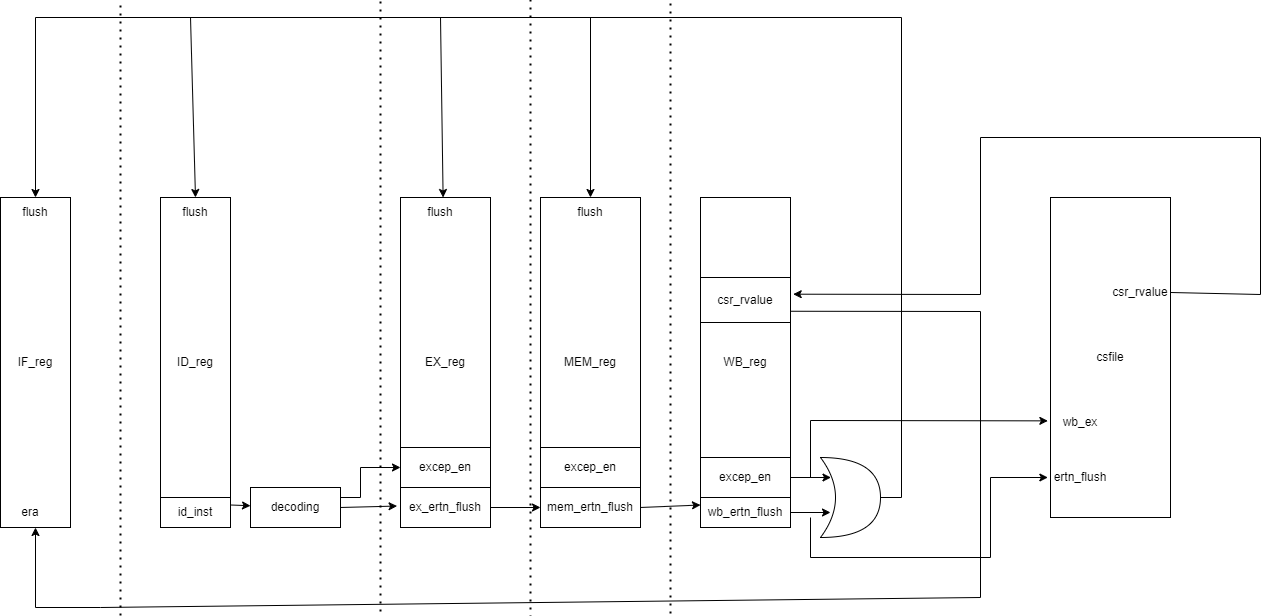
\includegraphics[width=0.9\textwidth]{./fig/fig1.png}
  \caption{syscall和ertn增加的部分数据通路}
\end{figure}
每个流水级,接受到清空流水线的信号时,将当前流水级的valid置0。

在IF流水级,如果接受到清空流水线的信号,将下一个pc值设置为从wb传来的返回的异常处理地址。
\begin{lstlisting}[language=verilog]
  assign pre_pc           =   flush ? wb_csr_rvalue // 将下一个pc值设置为从wb传来的返回的异常处理地址
                            : br_taken ? br_target 
                            : seq_pc;
\end{lstlisting}

\item  添加取指地址错(ADEF)、地址非对齐(ALE)、断点(BRK)和指令不存在(INE)异常的支持

从每个例外对应的判断阶段开始,其和其之后的每个阶段都添加一个1位宽的用于记录该条指令是否发生该种例外的控制信号。\par
ADEF在pre-IF级进行判断,当取值地址不为4字节对齐时,产生ADEF例外,并在WB阶段把错误地址传给BADV寄存器。
\begin{lstlisting}[language=verilog]
    assign pre_if_excep_ADEF   =     pre_pc[0] | pre_pc[1];   // 记录该条指令是否存在ADEF异常
    assign pre_if_excep_en =        pre_if_excep_ADEF;
\end{lstlisting}
INE和BRK均在ID阶段判断,当发现是相应指令时产生例外。
\begin{lstlisting}[language=verilog]
// 中断,系统调用,断点,指令不存在异常处理
    assign id_excep_INT     =   has_int;        // 记录中断信号
    assign id_excep_SYSCALL =   inst_syscall;   // 记录该条指令是否存在SYSCALL异常
    assign id_excep_BRK     =   inst_break;     // 记录该条指令是否存在BRK异常
    assign id_excep_INE     =   no_inst;        // 记录该条指令是否存在INE异常
    assign id_excep_en =        id_excep_INT | id_excep_SYSCALL | id_excep_BRK | id_excep_INE | if_excep_en;         //只要有一个异常就置1
    assign id_excep_esubcode =  9'h0;
\end{lstlisting}
ALE在EX阶段判断,当取半字时地址最低位为1,或取字时地址最后两位不全为0,则产生ALE例外,并记录错误地址,等到WB阶段将其传给BADV寄存器。
\begin{lstlisting}[language=verilog]
// 地址非对齐异常处理
    assign ex_excep_ALE = (ex_op_st_ld_h & ex_alu_result[0]) | (ex_op_st_ld_w & (ex_alu_result[1] | ex_alu_result[0]));     // 记录该条指令是否存在ALE异常
    assign ex_excep_en = ex_excep_ALE | id_excep_en;
    
    assign ex_vaddr = {32{ex_read_counter && ~ex_read_counter_low}} & counter[63:32] | 
                      {32{ex_read_counter && ex_read_counter_low}}  & counter[31: 0] |
                      {32{~ex_read_counter}} & ex_alu_result;
\end{lstlisting}

\item 计数器的添加

添加counter.v文件,存放计数器Stable\_Counter,没经过一个时钟周期自增1。
\begin{lstlisting}[language=verilog]
always @(posedge clk)begin
    if(~resetn)
        time_counter <= 64'b0;
    else
        time_counter <= time_counter + 1'b1;
end
\end{lstlisting}

\item 添加rdcntvl.w、rdcntvh.w和rdcntid指令

添加控制信号id\_read\_counter, id\_read\_counter\_low, id\_read\_TID,分别用于记录指令是否需要读取计数器的值,是否要读取计数器的低32位,指令是否要读取计数器ID。
\begin{lstlisting}[language=verilog]
    assign id_read_counter     = inst_rdcntvl_w | inst_rdcntvh_w;
    assign id_read_counter_low = inst_rdcntvl_w;
    assign id_read_TID         = inst_rdcntid; 
\end{lstlisting}
计数器的值在EX阶段根据ex\_read\_counter\_low完成读入。
\begin{lstlisting}
// 读计数器
    assign ex_counter_result = ex_read_counter_low ? counter[31:0] : counter[63:32];            //处理rdcntvl.w rdcntvh.w指令
\end{lstlisting}
TID的值在WB阶段完成读入。
\begin{lstlisting}
    assign final_rf_wdata = wb_csr_re   ? csr_rvalue : 
                            wb_read_TID ? csr_rvalue : wb_rf_wdata;             //add csr_tid_rvalue for rdcntid.w
\end{lstlisting}

\end{enumerate}


\vspace{1ex}

\section{实验过程中遇到的问题、对问题的思考过程及解决方法(比如RTL代码中出现的逻辑bug,逻辑仿真和FPGA调试过程中的难点等)}

\noindent
$\bullet$
\textbf{wb流水级的flush有效信号只持续一个clk}。

在清空流水线的设计时,将wb流水级在发出flush信号时的下一个clk时,也要将wb\_valid置为0,避免重复清空流水线。

使得如果IF流水级的allowin由于读后写数据相关等原因为0时,不能及时把\verb|pre_pc = wb_csr_rvalue| 发送给\verb|inst_sram|,而随着下一个clk的wb\_valid拉低,
使从wb传到if的wb\_csr\_rvalue信号也失效。

在这种情况下,不能正确地进行跳转到异常处理地址。

在分析波形图后,确定上述bug后,为if\_allowin添加上规则,使得接收到清空流水线时,立马将allowin拉高,在当前clk发送出pc

\begin{lstlisting}[language=verilog]
  assign if_allowin       =   ~if_valid               // valid是reg类型,接受flush后最快下一个clk才能拉低
                              | if_ready_go & id_allowin    // id_allowin可能由于读后写阻塞,拉低
                              | flush;    // 添加上规则,立马将allowin拉高,在当前clk发送出pc
\end{lstlisting}



\vspace{1ex}

\section{小组成员分工合作情况}
王敬华负责

李霄宇负责

艾华春负责exp12:添加系统调用异常支持

实验报告为根据每人负责代码的部分,写相应部分的报告。
\end{document}